

\section{EDAM}
    Το άρθρο "\textit{EDAM: An ontology of bioinformatics operations, types of data and identifiers, topics and formats}" των Ison, Kalas, Jonassen κ.α. πραγματεύεται την οντολογία EDAM, μια οντολογία που έχει σχεδιαστεί για την κατηγοροποίηση πράξεων και τύπων δεδομένων στην βιοπληροφορική. \cite{EDAMpaper}
    Η EDAM (EMBRACE Data and Models) είναι μια οντολογία από έννοιες που είναι διαδεδομένες στην ανάλυση βιοεπιστημονικών δεδομένων, περιλαμβάνει πράξεις (operations), τύπους δεδομένων (data types), data identifiers και data formats, όπως επίσης και συνώνυμα, συναφείς όρους, ορισμούς και άλλες πληροφορίες, όλα οργανωμένα με ιεραρχικό τρόπο. \cite{EDAMsite}

    \subsection{ΠΡΟΕΚΤΑΣΗ: Τι είναι η οντολογία;}
        Γενικά οντολογία είναι μια επίσημη αναπαράσταση γνώσης σε ένα συγκεκριμένο πεδίο.
        Ορίζει ένα σύνολο εννοιών και κανόνων όπως επίσης και τις μεταξύ τους σχέσεις σε ένα δομημένο format που μπορεί να διαβαστεί εύκολα και από της μηχανές.
        Υπάρχει ιεράρχηση στις έννοιες μέσω της δημιουργίας κλάσεων, ιδιότητες (attributes) από αυτές τις έννοιες, σχέσεις (relationships) μεταξύ τους όπως επίσης και παραδείγματα (instances) από τις έννοιες.
        Μια οντολογία αναπαρίσταται σε γλώσσες σήμανσης όπως η OWL (Web Ontology Language) ή RDF (Resource Description Framework XML), γλώσσες που έχουν βασιστεί πάνω στην XML. \cite{OntologyWiki} \cite{BioOntologies}

    \subsection{Πώς δημιουργήθηκε η ανάγκη για να δημιουργηθεί η οντολογία EDAM;}
        Σε μια εποχή ταχείας ανάπτυξης της βιολογίας και της πληροφορικής με αποτέλεσμα την αύξηση των πληροφοριακών αναγκών, μέχρι πρότινος δεν υπήρχε μια ολοκληρωμένη οντολογία με σωστές ταξινομημένες πληροφορίες κατά ένα τρόπο που να υποστηρίζονται πράξεις μεγάλης κλίμακας.
        Τα λεξικά και οι οντολογίες που είχαν δημιουργηθεί ως τότε δεν κάλυπταν πλήρως τις ανάγκες που απαιτούσε η επιστήμη της βιοπληροφορικής.

    \subsection{Τι προσφέρει η οντολογία EDAM;}
        Η οντολογία EDAM σχεδιάστηκε με γνώμονα να είναι σχετική με τις προβλεπόμενες εφαρμογές της στη βιοπληροφορική.
        Για να επιτευχθεί αυτό, μελετήθηκαν οι υπάρχουσες οντολογίες και εργαλεία (myGrid ontology (2007), εργαλεία από την EMBRACE, BioMoby Object Ontology (2001)).
        Ακολουθούνται αρχές όπως η λογική συνέπεια (να μην υπάρχουν αντιφάσεις στην οντολογία), σαφές σημασιολογικό πεδίο (είναι καθορισμένα τα όρια του τι καλύπτει) όπως επίσης και η δυνατότητα για μελλοντικές προεκτάσεις.

    \subsection{Υλοποίηση EDAM}
        Η οντολογία χρησιμοποιεί URIs (Uniform Resource Identifiers) για τη μοναδική αναπαράσταση των εννοιών της, με τη μορφή: \verb|http://e-damontology.org/<subontology>_<localId>|.

        Υπάρχουν τέσσερις διαφορετικές υποοντολογίες: \textbf{Operation} (συνάρτηση με εισόδους και εξόδους, πχ πρόβλεψη δομής RNA), \textbf{Data} (πληροφορία, πχ αλληλουχίες) και τη δική του υπακολουθία \textbf{Identifier}, \textbf{Topic} (περιγράφει κατηγορίες, πχ <<Ανάλυση αλληλουχιών>>) και \textbf{Format} (μορφές δεδομένων, πχ FASTQ).
        Έτσι, η κλάση <<Sequence record>> για παράδειγμα αναπαρίσταται ως \verb|http://edamontology.org/data_0849|. \linebreak
        Οι σχεσιακές σχέσεις και οι υπόλοιπες ιδιότητες ορίζονται με τη μορφή: \verb|http://edamontology.org/<id>|.

        \begin{figure}[h!] \noindent\centering
            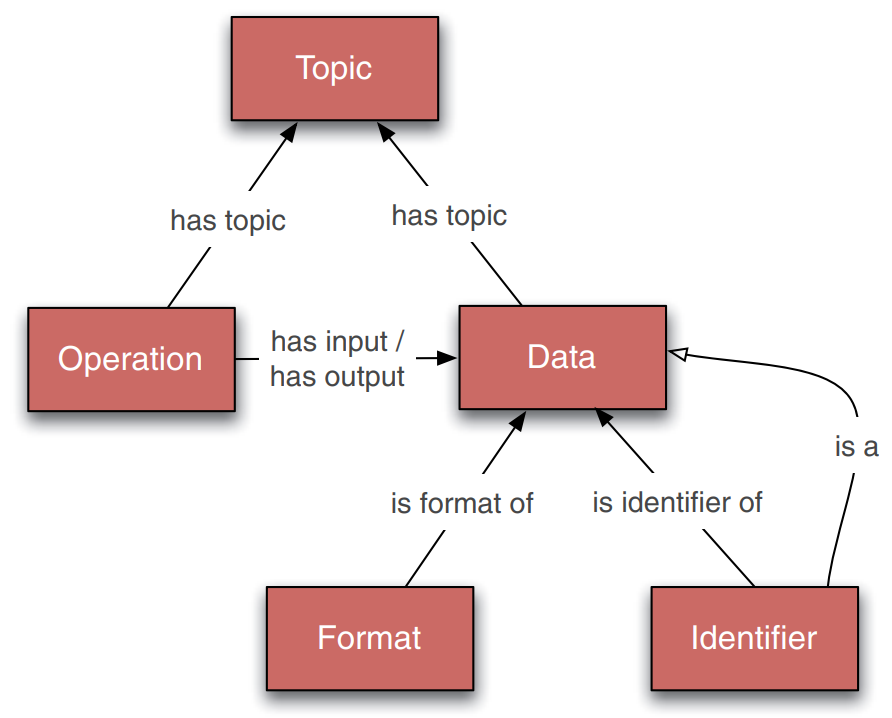
\includegraphics[scale=0.4]{img/Edam subontologies}
            \caption{Σχέσεις μεταξύ των υποοντολογιών \cite{EDAMpaper}}
        \end{figure}

% Παράγραφος 3.2
% Παραπάνω πληροφορίες για προηγούμενες οντολογίες (myGrid, BioMoby).


\section{METATRON}

\section{ΤΕΛΕΥΤΑΙΟ PAPER}